Das Diagramm zeigt den Ort $s$ eines Körpers, der sich auf einer geraden Linie bewegt.
\begin{center}
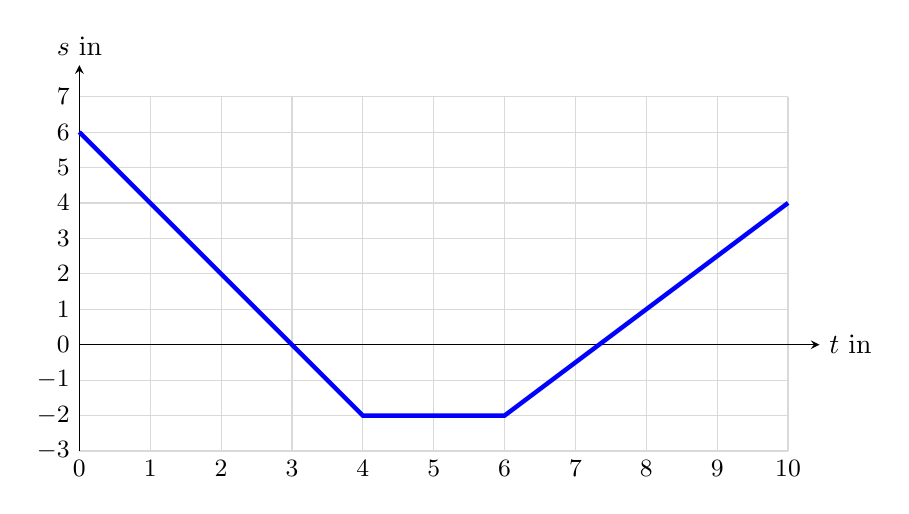
\begin{tikzpicture}[>=stealth, x=0.9cm, y=0.45cm]
 \draw[gray!30] (0,-3) grid[xstep=1, ystep=1] (10,7);
 \draw[->] (0,0) -- (10.444,0) node[right] {$t$ in \si{\second}};
 \draw[->] (0,-3) -- (0,7.889) node[above] {$s$ in \si{\meter}};
 \foreach \tk in {0,1,2,3,4,5,6,7,8,9,10} \node[below] at (\tk,-3) {\small $\tk$};
 \foreach \yk in {-3,-2,-1,0,1,2,3,4,5,6,7} \node[left] at (0,\yk) {\small $\yk$};
 \draw[ultra thick, blue] (0,6) -- (4,-2) -- (6,-2) -- (10,4);
\end{tikzpicture}
\end{center}
\begin{abcliste}
\abc In welchen Zeitabschnitten ist die Geschwindigkeit negativ, null bzw. positiv?
\abc \DuSie{Bestimme}{Bestimmen Sie} die Geschwindigkeit von \SI{0}{\second} bis \tOneO\ und von \tTwoO\ bis \tEndO.
\abc Mia meint: „Von \tTwoO\ bis etwa \SI{7.3}{\second} ist die Geschwindigkeit negativ, weil der Körper dort im negativen Bereich ist.“ Was \DuSie{sagst du}{sagen Sie} dazu?
\end{abcliste}
